\section{问题三：垂荡--纵摇四自由度响应求解}

\subsection{非线性几何耦合模型}

\begin{figure}[H]
  \centering
  % 左图，占0.45行宽
  \begin{minipage}{0.45\textwidth}
    \centering
    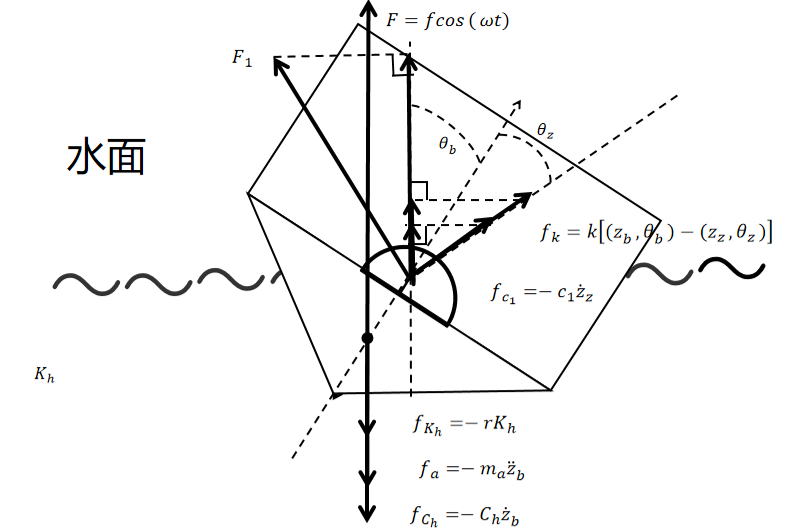
\includegraphics[width=\linewidth]{fig_problem3_xiugai.png}
    \subcaption{振子}
  \end{minipage}
  \hfill
  \begin{minipage}{0.45\textwidth}
    \centering
    
\includegraphics[width=\linewidth]{fig_problem3_model4.png}
    \subcaption{浮子}
  \end{minipage}
  % 总图题
  \caption{系统受力分析}
  \label{fig:raw_resample3}
\end{figure}

\begin{figure}
    \centering
    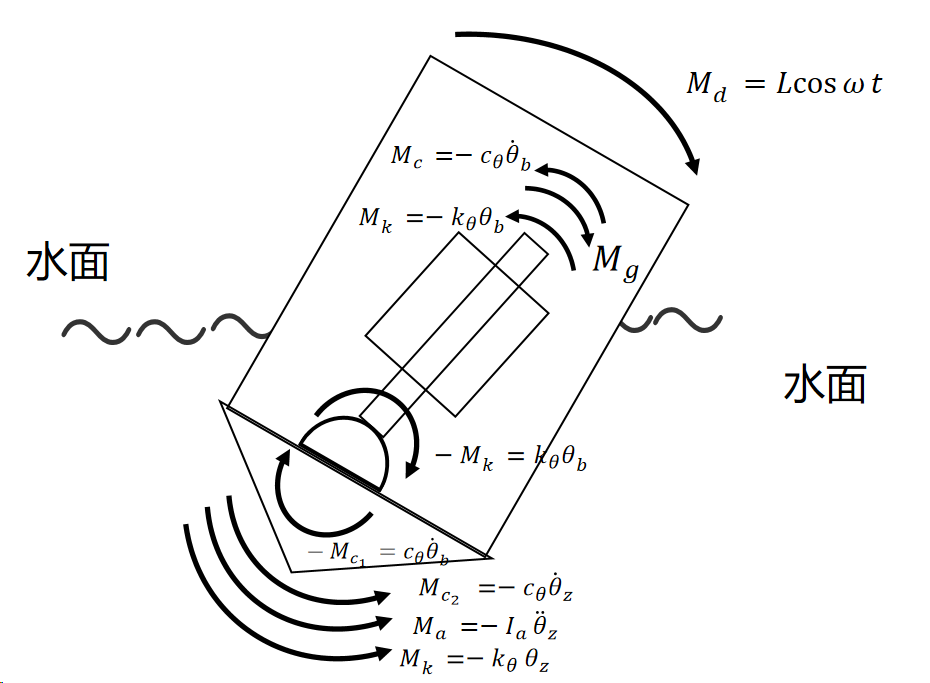
\includegraphics[width=0.75\linewidth]{fig_problem3_model5.png}
    \caption{力矩分析}
    \label{fig:placeholder6}
\end{figure}
问题三加入旋转阻尼器和扭转弹簧后，系统状态取为
\[
  \bm{x}=(z_z,z_b,\theta_z,\theta_b,\dot z_z,\dot z_b,\dot\theta_z,\dot\theta_b)^\mathsf{T}.
\]
其中 $z_z$ 表示振子沿浮子中轴方向的位置，$z_b$ 表示浮子垂荡位移，$\theta_z$ 表示振子相对浮子的纵摇角，$\theta_b$ 表示浮子纵摇角。振子中轴与竖直方向的夹角为
\[
  \phi=\theta_z+\theta_b .
\]

\iffalse
\begin{figure}[H]
  \centering
  % 左图，占0.45行宽
  \begin{minipage}{0.45\textwidth}
    \centering
    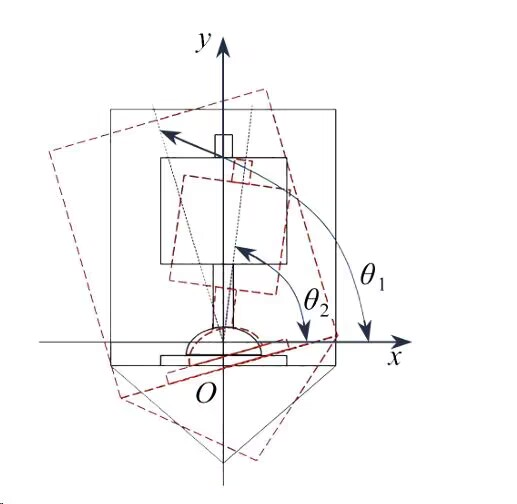
\includegraphics[width=\linewidth]{fig_problem3_model2.jpg}
    \subcaption{振子}
  \end{minipage}
  \hfill
  \begin{minipage}{0.45\textwidth}
    \centering
    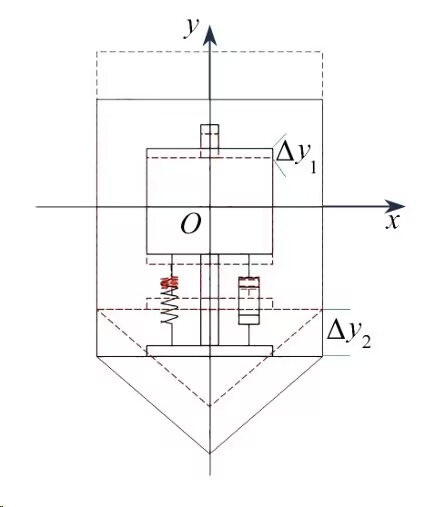
\includegraphics[width=\linewidth]{fig_problem3_model3.jpg}
    \subcaption{浮子}
  \end{minipage}
  % 总图题
  \caption{力矩分析}
  \label{fig:raw_resample2}
\end{figure}
\fi

浮子纵摇角加速度由力矩平衡给出：
\begin{equation}
  \ddot\theta_b=
  \frac{-K_\theta\theta_b-C_\theta\dot\theta_b+c_2\dot\theta_z
  +k_\theta\theta_z+L\cos\omega t}{I_b+J_a}.
  \label{eq:theta_b}
\end{equation}
振子相对纵摇的转动惯量随滑移位置变化：
\begin{equation}
  I_z^\ast=I_z+m_zz_z^2,
\end{equation}
对应角加速度为
\begin{equation}
  \ddot\theta_z=
  \frac{-c_2\dot\theta_z-k_\theta\theta_z+m_zgz_z\sin\phi}{I_z^\ast}
  -\ddot\theta_b .
  \label{eq:theta_z}
\end{equation}

垂荡方向上，浮子等效质量包含几何耦合项 $m_z\sin^2\phi$。在保留 AProblem 附录中惯性耦合项的形式下，可写为
\begin{equation}
  \ddot z_b=\frac{\mathcal{F}_b(z_z,z_b,\theta_z,\theta_b,\dot z_z,\dot z_b,\dot\theta_z,\dot\theta_b,t)}
  {m_b+m_a+m_z\sin^2\phi},
\end{equation}
其中 $\mathcal{F}_b$ 包含弹簧分力、阻尼分力、兴波阻尼、静水恢复力、波浪激励力以及振子垂直中轴方向惯性力。振子沿中轴方向加速度由
\begin{equation}
  \ddot z_z=\frac{-k(z_z-l_0)-c_1\dot z_z-m_zg\cos\phi
  -m_z\mathcal{A}_r}{m_z}
\end{equation}
给出，其中 $\mathcal{A}_r$ 为由浮子垂荡加速度和两角速度产生的径向惯性耦合项。

\subsection{求解设置与结果}

第三问中题给阻尼参数取 $c_1=10000\,\mathrm{N\cdot s/m}$、$c_2=1000\,\mathrm{N\cdot m\cdot s}$。由于方程含有较强非线性耦合并具有一定刚性，本文采用 Radau 隐式积分方法，误差控制为相对容差 $10^{-8}$、绝对容差 $10^{-10}$。初始条件取浮子处于静水平衡，振子沿中轴方向位于弹簧静平衡长度
\[
  z_z(0)=l_0-\frac{m_zg}{k}.
\]

\begin{figure}[H]
  \centering
  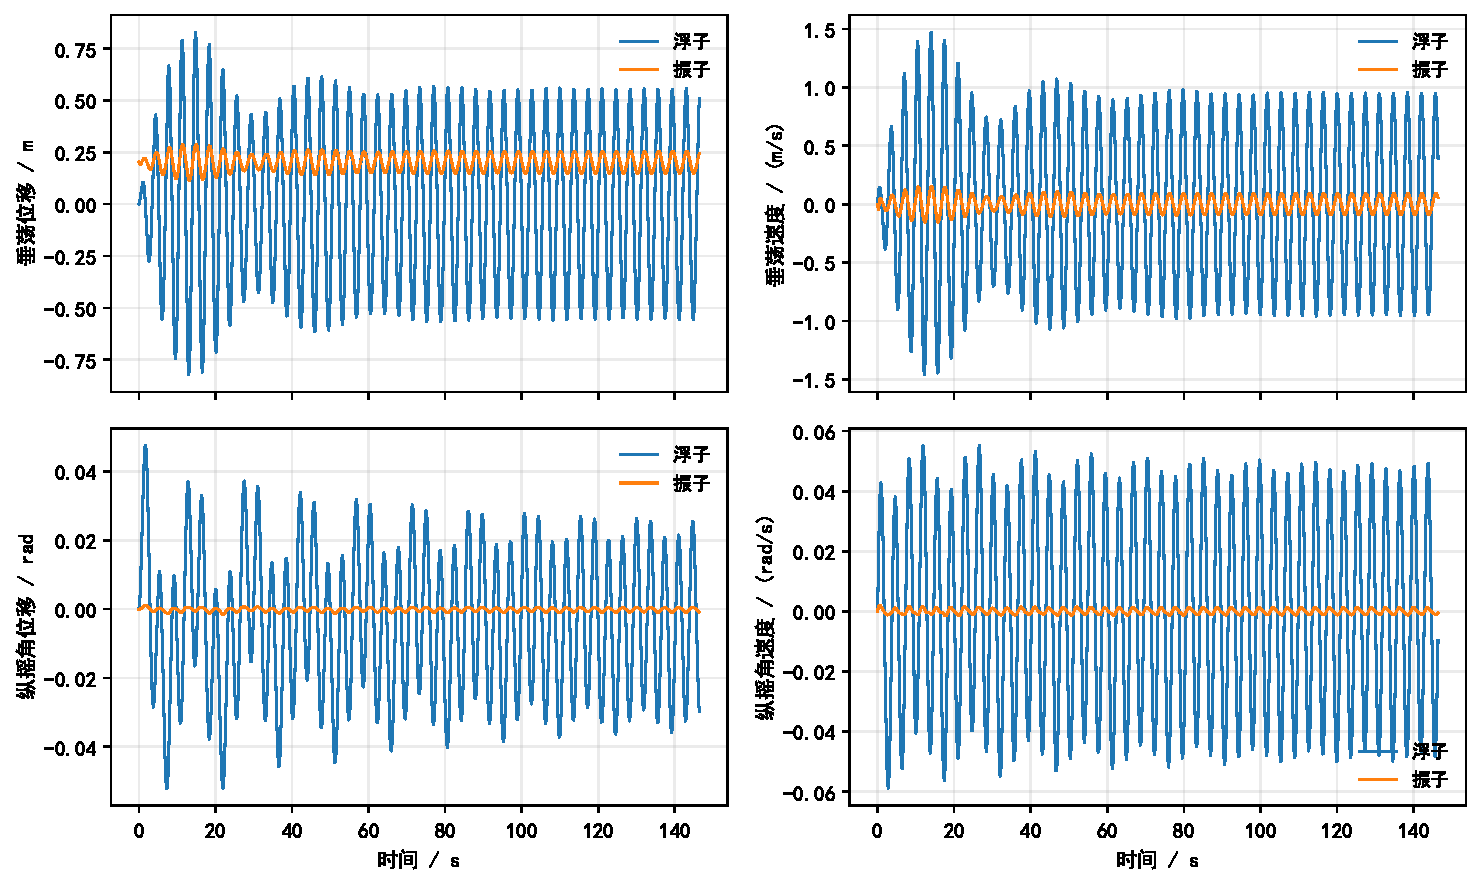
\includegraphics[width=0.95\textwidth]{fig_problem3_response.pdf}
  \caption{问题三给定阻尼参数下的四自由度响应}
  \label{fig:p3_response}
\end{figure}

\begin{figure}[H]
    \centering
    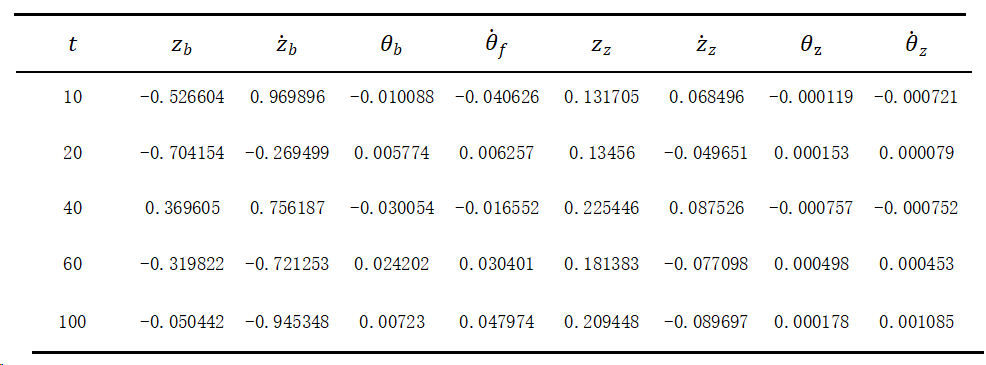
\includegraphics[width=0.9\linewidth]{fig_problem3_data.png}
    \caption{几个时间点的相关数据}
    \label{fig:placeholder4}
\end{figure}

由图~\ref{fig:p3_response} 可见，浮子垂荡响应幅值显著大于振子沿轴滑移幅值；纵摇响应中浮子角位移明显大于振子相对角位移。该结果说明在题给参数下，纵摇运动存在但幅值较小，后续功率优化中旋转阻尼功率可能不会成为总功率主导项。
